\documentclass[a4paper, 12pt, notitlepage]{report}

\usepackage{amsfonts} % if you want blackboard bold symbols e.g. for real numbers
\usepackage{graphicx} % if you want to include jpeg or pdf pictures
\usepackage{pdfpages}

\title{Exam Invigilator Communications System\\
Interim Report} % change this
\author{Richard CB Evans\\
Department of Electrical and Electronic Engineering\\
Imperial College London} % change this
\date{\today} % change this

\begin{document}

\maketitle
\begin{center}
Supervised by Dr.\ Mark Wheelhouse. % change this
\end{center}
\thispagestyle{empty}
\newpage

\tableofcontents 

\chapter{Introduction}
%
Despite the high uptake of technology through the university education system, one aspect remains very manual: Exam Invigilation.

During each exam session, it is common to have invigilators spread across multiple rooms, either due to the popularity of certain courses, timetable collisions, or having students with extra time.

There are many reasons for which invigilators may need to communicate during these sessions.  For example, examination start and finish times need to be coordinated, clarifications or corrections need sharing amongst exam rooms, and students may need escorting to the bathroom.  This can be particularly troublesome for rooms with single invigilators.

Whilst most invigilators carry a mobile phone which could be used for communicating with other rooms, this is not a reliable solution to the communication issue.  Not all invigilators do carry a phone, and invigilators do not necessarily know the number of all other invigilators in other rooms.  Furthermore, it is necessary for all mobile phones to be placed in silent mode, leading to communications being missed.

Improving ease and speed of communication between exam invigilators is highly desirable as, ultimately, it will improve the quality of the student exam experience.  Quick and efficient communication will mean problems can be identified, shared and resolved more quickly, meaning students can receive corrections, visit the bathroom or obtain more paper sooner.  This allows the students to spend their time focussed on the task at hand; answering the paper in front of them.

The project is to create an easy to use and effective real-time communication system.

\chapter{Background}
%
In this chapter I will describe the background research done before any design or implementation decisions were made.

\section{System Requirements}

In this section I will describe the initial investigation done to establish the requirements of the system.

\subsection{Initial Research}

Before beginning development, it was essential to identify the requirements of the system additional to those outlined in the project specification.  Ultimately, the success of the system would be judged by those it was intended for; invigilators, and so I approached and interviewed an Imperial Department of Computing invigilator to establish the aspects of a prospective system which would influence his opinion of its success.

A number of areas were identified:

\begin{itemize}
\item Ease of Use\\
The interface must be simple enough to operate quickly and accurately.
\item Security\\
Examination information is often confidential and so access must be restricted to those  with the appropriate permissions.
\item Reliability\\
Exams are critical components of the university education process and so it is imperative that any computerised system would be completely reliable.  All information must be shared in real-time and shared with any and all necessary members of staff.  Any cause to resort to traditional communication methods would render the system a failure.
\item Discretion\\
The operation of the communication system must not disturb the students who are being examined in the room.  It is, however, important that the system be effective at drawing the users attention to any alerts and messages broadcast, to avoid information being missed.
\item Functionality\\
There are a certain number of functionalities which the system must offer to be considered useful to those invigilating:

\begin{itemize}
\item Show at a glance which room(s) need assistance.
\item Allow an invigilator to notify others when the exam(s) in their room have started or stopped.
\item Request an examiner come to their room, for example to answer a student's question.
\item Request assistance from another invigilator, for example to escort a student to the bathroom.
\item The requesting invigilator is able to see that someone is on the way to help, however, it is important that this information is shared such that a room is not over-serviced.
\item Broadcast an announcement to be made in all rooms of a certain exam, with acknowledgement of receipt.
\end{itemize}
\end{itemize}

\subsection{Further Research}

With the initial requirements discussed with an invigilator, I made the decision to reach out to other invigilators for more input with a short web survey which was shared via e-mail to the Department of Computing alias for all teaching fellows.  I also received interest from the Electrical and Electronic Engineering department and so shared the survey with the staff there to gather more opinions and information to assist with the direction the project should take.

The full results of the web survey can be found in appendix A.

\subsection{Research Results Analysis and Requirements}

In the online survey answered by the staff of both the Department of Computing and Electrical and Electronic Engineering, I asked a number of questions regarding the preference of device and feature specification.

By far the most prolific devices were phones running the Android operating system, owned by half of all respondents, followed by the iPhone, owned by 20\%.  iPhone combined with the iPad made up 9 devices owned by staff, with Android phones and tablets making 15.

When offered the choice of using an Android powered device, owned by the Department of Computing, or using their own device, 58\% of respondents indicated a preference of using a provided departmental device, however, when asked whether they would prefer the system to use a web interface or be a native application, 62\% indicated that they would prefer a web interface, with 12.5\% preferring a native application.

The preference for a web interface was discussed during the initial interview where, it was expressed that a native application running on a departmental tablet device would be best.  Whilst many invigilators take a laptop to exams, they generally spend the time working in full screen applications.  As a result, if a web interface were to be implemented for the system, they would likely have the system open in a background browser window while they work.  This would make any attempt at notifying of a message near impossible and would rely on them frequently checking the status of the system.  This would inconvenience them while they work, decreasing the likelihood of them checking regularly, making the system hard to justify.  Use of a tablet, however, would mean that extra functions such as a device vibrator and manipulation of the display could be used to attract attention of the invigilator and the device could also be left in a prominent position alongside them working to be seen.  This goes with the extra mobility of the device, allowing them to carry it whilst responding to students with raised hands, allowing them to advertise if assistance is needed instantly.  As a result, I have made the decision that an Android application should be the priority in development, with a web interface being a stretch goal that can be investigated if time permits as the project progresses.

The survey respondents were asked which information they felt it was important to have visible on the screen instantly accessible, and which functionality they felt would be important for a successful communication system.  The survey website attributed each response a value from 1-4 with increasing importance which was then divided by the number of respondents to give a response average value which the list could then be sorted by, as seen in the results tables in appendix A.  Respondents were further given the opportunity to give their own suggestions of functionality of notification methods.

\subsubsection{Core Functionality}

Having analysed the predetermined system requirements and the responses of all web survey respondents, the suggested features have been split into three functionality groups; the essential core functionality, and two stretch goal groups which can be attempted with sufficient time.  The system will be designed in such a way that inclusion of the stretch goal functionality will not require complete re-engineering of the core system.\\

Core Requirements:

\begin{itemize}
\item Allow Invigilators and Examiners to sign into the system and assign themselves to a specific room, or as floating staff

\item Provide the ability to update the room a user is in and reflect this change across the system

\item Offer a means of electronic text communication between invigilators and examiners
\begin{itemize}
\item Nature of Recipients
\begin{itemize}
\item Send to all
\item Send to all in specific room
\item Send to all examiners
\item Send to an individual
\end{itemize}
\item Nature of Message
\begin{itemize}
\item Preset generic assistance needed message
\item Preset specific assistance needed message, i.e. Bathroom Escort
\item Allow typing of custom messages
\end{itemize}
\item Acknowledgement of Message
\begin{itemize}
\item Provide a positive response to the individual requesting help
\item Dismiss notification on other users' screens so that the request is not over serviced
\item Append response to the communication log
\end{itemize}
\item Provide a log to browse the history of all communications
\end{itemize}

\item Allow users to view and control exam timings in their own room, and view the status of other rooms
\begin{itemize}
\item Exam start time
\item Time remaining
\item Exam finish time
\item Extra Time finish time
\end{itemize}

\item Provide a listing of active users on the system, and their locations.

\item Effectively alert users to new incoming messages in a way not distracting to students sitting the exam.

\end{itemize}

\subsubsection{Stretch Goals}

Beyond the core functionality specified above, the remaining ideas for functionality can be split into two categories of decreasing importance.  These requirements differ from the core list in that if not successfully implemented into the system, the system could be deemed a success as inter invigilator/examiner communication will be possible.

In the case that the project progresses in good time ahead of schedule, first group 1 then group 2 stretch goals will be implemented.

\begin{enumerate}
\item More Important
\begin{itemize}
\item Include information for each examination, including the examiner responsible for asking each question of a paper.
\item Include critical contact numbers for each exam paper.
\item Provide student seating plans mapping student names to numbers, and vice versa.
\item The ability to customize notification methods, e.g. Toggle device vibration on message received.
\end{itemize}

\item Less Important

\begin{itemize}
\item Implement a client web interface for the system.
\item Include additional information such as student ID photo in student list.
\item Add the ability to scan student IDs to automate up the ID checking process.
\item Use of the system to replace current pen and paper administration such as student count.
\end{itemize}
\end{enumerate}

\section{Available Data}

In the Department of Computing, all examination information and timetables, seating plans and invigilation schedules are already computerised and available via internal APIs.  This project will seek to build upon these available APIs to fetch and receive information as required, for example, to find the examiner for a specific question on a paper.

If it is found that the available APIs are incapable of providing adequate levels of detail necessary for the desired functionality of the system, I will engage with the Department to discuss the possibility of extending or improving the existing APIs, or investigate hosting information central to the Communication system which can then expose APIs for external use instead, if necessary.

\subsection{Confidentiality of Data}

As previously stated, the exam scheduling, seating plans and invigilator information contains sensitive data protected by the data protection act.  As a result, during the development of the system, I will make use of mock data.

\section{Existing Infrastructure}

\subsection{Server Hosting}
As it is necessary to centralise access to the existing APIs offering information about the exam timetables and other information, it will be necessary to make use of a server to which clients can connect and which hosts the information about ongoing exams.  Use a central server will also avoid complexities associated with peer to peer network discovery and communication.

Imperial College offers a Virtual Cloud Server Hosting service providing the ability for staff and members of research groups to provision their own virtual servers on demand for hosting their specialised applications.

The servers can be provisioned with either Windows Server or Redhat Enterprise Linux distributions.  Full administrative privileges are granted to the user providing complete control over the install and configuration of the system as required. 

\subsection{Network Communication}

The Department of Computing is already fitted with a widely accessible wireless local area network which interfaces the Virtual Cloud Server hosting.  Client server connection will therefore be possible via connection to the Imperial-WPA wifi connection, or via VPN.

\subsection{System Security}

Given the nature of the information to be made available in the exam invigilator communication system, it is necessary that the system features restricted access to only authorised members of the college faculty involved with the invigilation or examination of the exams.

\chapter{Project Plan}
%

\chapter{Evaluation Plan}
%

\appendix
\chapter{Web Survey Results}

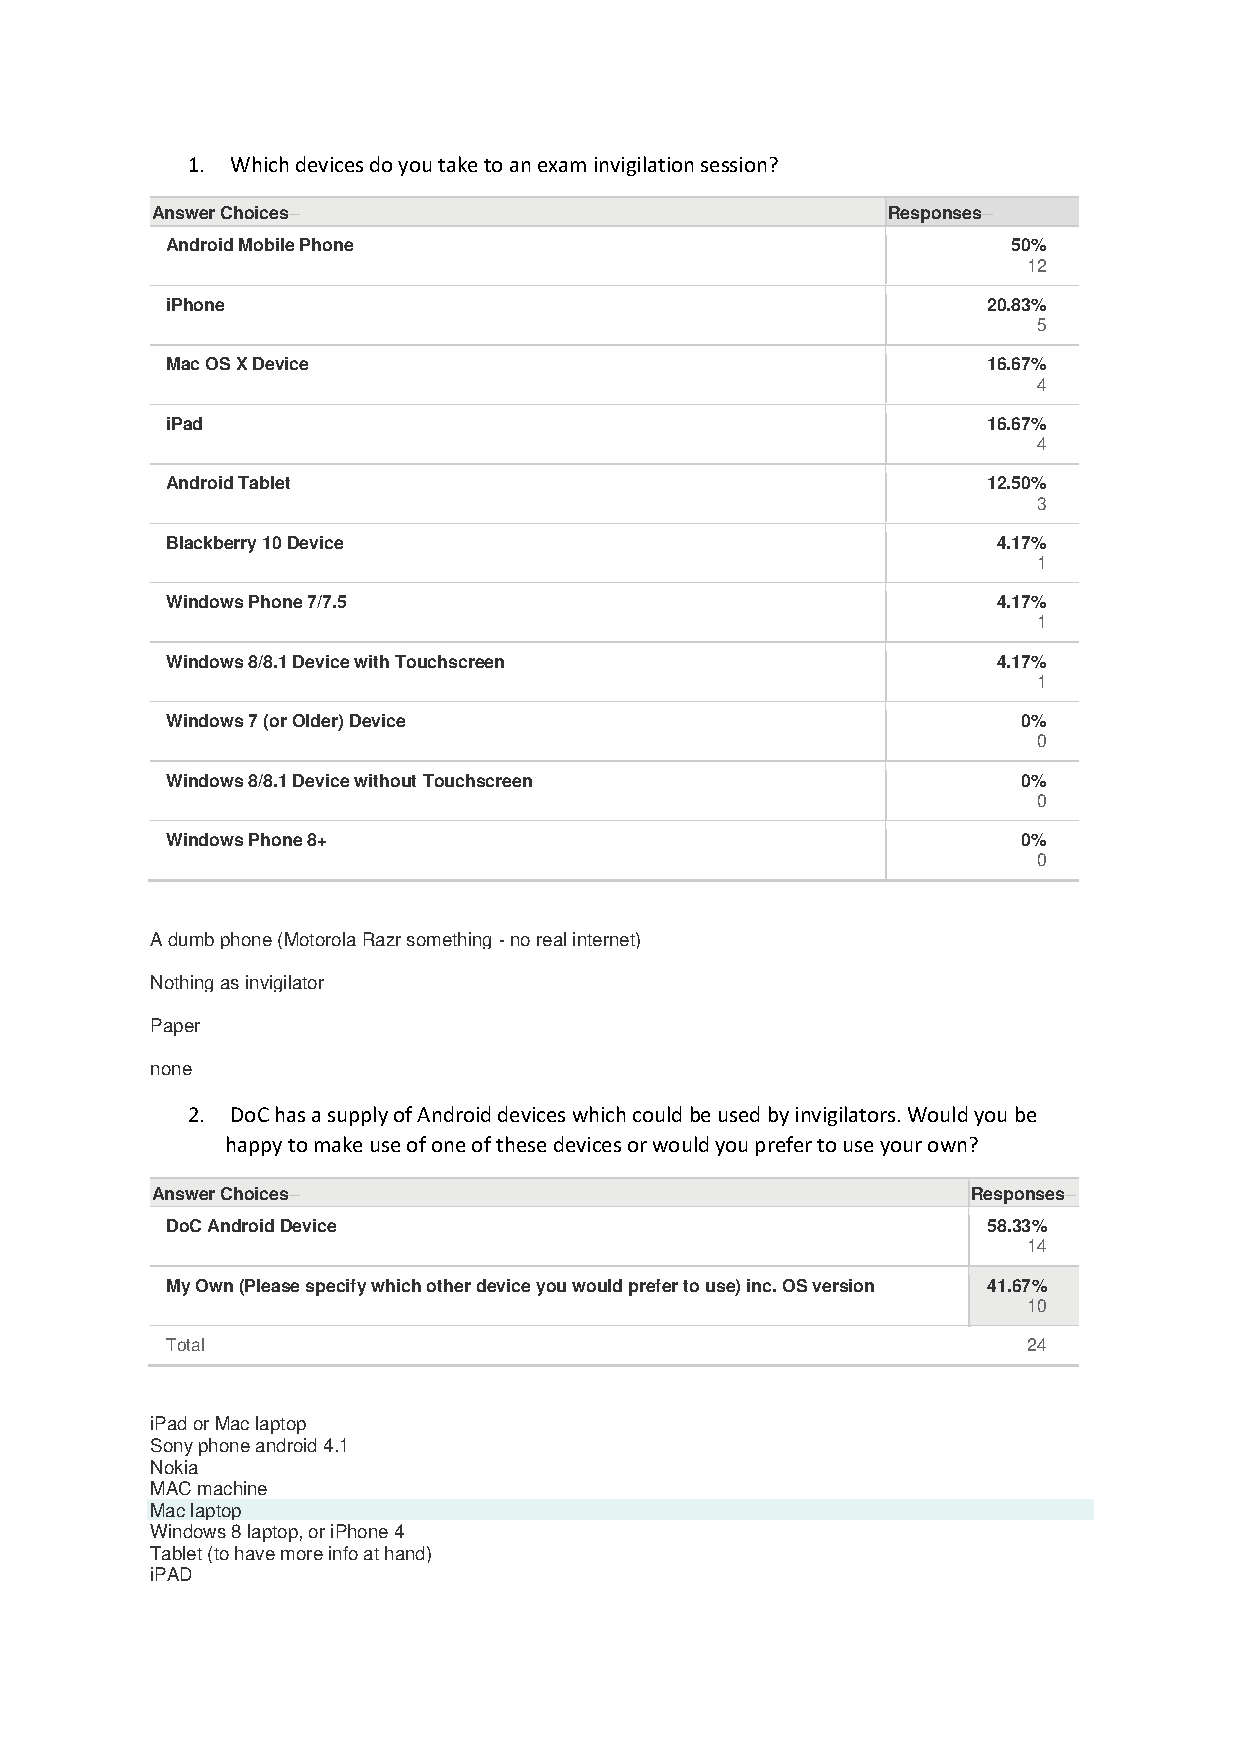
\includepdf[pages=-]{surveyResult.pdf}

%%%%%%%%%% BIBLIOGRAPHY %%%%%%%%%%
\chapter*{Bibliography}
%
\begin{description}

\item Author, I. (Year). \emph{Book Title}, Publisher; Place of publication.

\item Lamport, L. (1986), \emph{\LaTeX: A Document Preparation System}, Addison-Wesley; Reading, MA.

\item Author, I. (Year). `Journal article title', \emph{Journal}, \textbf{Vol}, pp.first--last.

\item Smith, A.D.A.C. and Wand, M.P. (2008). `Streamlined variance calculations for semiparametric
mixed models', \emph{Statistics in Medicine}, \textbf{27}, pp.435--48.

\end{description}

\end{document}